\documentclass[manuscript, letterpaper]{aastex6}

% to-do list
% ----------
% - check for TODO's and references to APW, HOGG, SMOH
% style notes
% -----------
% - This file generates by Makefile; don't be typing ``pdflatex'' or some bullshit.
% - Line break between sentences to make the git diffs readable.
% - Use \, as a multiply operator.
% - Reserve () for function arguments; use [] or {} for outer shit.
% - Use \sectionname not Section, \figname not Figure, \documentname not Article or Paper or paper.

\include{gitstuff}
% ----------------------------------- %
% start of AASTeX mods by DWH and DFM %
% ----------------------------------- %

\setlength{\voffset}{0in}
\setlength{\hoffset}{0in}
\setlength{\textwidth}{6in}
\setlength{\textheight}{9in}
\setlength{\headheight}{0ex}
\setlength{\headsep}{\baselinestretch\baselineskip} % this is 2 lines in ``manuscript''
\setlength{\footnotesep}{0in}
\setlength{\topmargin}{-\headsep}
\setlength{\oddsidemargin}{0.25in}
\setlength{\evensidemargin}{0.25in}

\linespread{0.54} % close to 10/13 spacing in ``manuscript''
\setlength{\parindent}{0.54\baselineskip}
\hypersetup{colorlinks = false}
\makeatletter % you know you are living your life wrong when you need to do this
\long\def\frontmatter@title@above{
\vspace*{-\headsep}\vspace*{\headheight}
\noindent\footnotesize
{\noindent\footnotesize\textsc{\@journalinfo}}\par
{\noindent\scriptsize Preprint typeset using \LaTeX\ style AASTeX6
with modifications by DWH and DFM.
}\par\vspace*{-\baselineskip}\vspace*{0.625in}
}%
\long\def\frontmatter@abstractheading{%
\makeaffils
  \vspace*{-\baselineskip}\vspace*{1.5pt}
  \vspace*{0.13189in}
 \begingroup
  \centering
  \abstractname
  \vskip 1mm
  \par
 \endgroup
 \everypar{\rightskip=0.0in\leftskip=\rightskip}\par
}%
\def\frontmatter@keys@format{\vspace*{0.5mm}%
  \settowidth{\keys@width}{\normalsize\@keys@name}%
  \rightskip=0.0in\leftskip=\rightskip\parindent=0pt%
    \hangindent=\keys@width\hangafter=1\normalsize\raggedright}%
\def\twodigits#1{\ifnum#1<10 0\fi\the#1}
\def\mydate{\leavevmode\hbox{\the\year-\twodigits\month-\twodigits\day}}
\makeatother
\renewcommand{\today}{\mydate}

% Section spacing:
\makeatletter
\let\origsection\section
\renewcommand\section{\@ifstar{\starsection}{\nostarsection}}
\newcommand\nostarsection[1]{\sectionprelude\origsection{#1}}
\newcommand\starsection[1]{\sectionprelude\origsection*{#1}}
\newcommand\sectionprelude{\vspace{1em}}
\let\origsubsection\subsection
\renewcommand\subsection{\@ifstar{\starsubsection}{\nostarsubsection}}
\newcommand\nostarsubsection[1]{\subsectionprelude\origsubsection{#1}}
\newcommand\starsubsection[1]{\subsectionprelude\origsubsection*{#1}}
\newcommand\subsectionprelude{\vspace{1em}}
\makeatother

\widowpenalty=10000
\clubpenalty=10000

\sloppy\sloppypar

% ------------------ %
% end of AASTeX mods %
% ------------------ %


% packages
\definecolor{cbblue}{HTML}{3182bd}
\usepackage{microtype}  % ALWAYS!
\usepackage{amsmath}
\hypersetup{backref,breaklinks,colorlinks,urlcolor=cbblue,linkcolor=cbblue,citecolor=black}

% define macros for text
\newcommand{\project}[1]{\textsl{#1}}
\newcommand{\acronym}[1]{{\small{#1}}}
\newcommand{\gaia}{\project{Gaia}}
\newcommand{\rave}{\project{\acronym{RAVE}}}
\newcommand{\apogee}{\project{\acronym{APOGEE}}}
\newcommand{\tmass}{\project{\acronym{2MASS}}}
\newcommand{\documentname}{\textsl{Article}}
\newcommand{\sectionname}{Section}
\newcommand{\figname}{Figure}
\newcommand{\eqname}{Equation}
\newcommand{\dr}{\acronym{DR1}}
\newcommand{\tgas}{\acronym{TGAS}}

% define macros for math
\newcommand{\given}{\,|\,}
\newcommand{\normal}{{\mathcal{N}}}
\newcommand{\dd}{\mathrm{d}}
\newcommand{\transp}[1]{{#1}^{\!\mathsf{T}}}
\newcommand{\inv}[1]{{#1}^{-1}}
\newcommand{\bs}[1]{\boldsymbol{#1}}
\newcommand{\vperp}{\bs{v}^\perp}
\newcommand{\propm}{\bs{\mu}}
\newcommand{\mat}[1]{\mathbf{#1}}
\renewcommand{\vec}[1]{\bs{#1}}
\newcommand{\kms}{\ensuremath{\rm km~s^{-1}}}
\newcommand{\msun}{{\rm M}_\odot}
\newcommand{\data}{\mathrm{data}}
\newcommand{\snr}{[S/N]_\varpi}
\newcommand{\eye}{\mathbb{I}}
\newcommand{\absdvtan}{\ensuremath{|\Delta\vec v_\mathrm{t}|}}

% TODO
\newcommand{\todo}[1]{{\color{red}TODO: #1}}

\begin{document}\sloppy\sloppypar\raggedbottom\frenchspacing % trust me

\title{Co-moving stars in \textsl{Gaia DR1}}
\author{Semyeong Oh\altaffilmark{\pu,\lead},
        Adrian M. Price-Whelan\altaffilmark{\pu},
        David W. Hogg\altaffilmark{\ccpp,\mpia,\cca},
        Timothy D. Morton\altaffilmark{\pu},
        David N. Spergel\altaffilmark{\pu,\cca}
}

% Affiliations
\newcommand{\pu}{1}
\newcommand{\lead}{2}
\newcommand{\ccpp}{3}
\newcommand{\mpia}{4}
\newcommand{\cca}{5}

\altaffiltext{\pu}{Department of Astrophysical Sciences,
                   Princeton University, Princeton, NJ 08544, USA}
\altaffiltext{\lead}{To whom correspondence should be addressed:
                     \texttt{semyeong@astro.princeton.edu}}
\altaffiltext{\ccpp}{Center for Cosmology and Particle Physics,
                     Department of Physics,
                     New York University, 4 Washington Place,
                     New York, NY 10003, USA}
\altaffiltext{\mpia}{Max-Planck-Institut f\"ur Astronomie,
                     K\"onigstuhl 17, D-69117 Heidelberg, Germany}
\altaffiltext{\cca}{Center for Computational Astrophysics, 162 5th Ave, New York, NY 10003, USA}

\begin{abstract}
% Context
The primary sample of the \gaia\ \textsl{First Data Release} is the brand-new
\textsl{Tycho-Gaia Astrometric Solution}. The precision and size of this sample
creates an opportunity to find new binary stars and moving groups, especially
rare binaries or sparsely populated groups.
% Aims
Here we seize this opportunity.
% Methods
We use a justified marginalized likelihood ratio test to separate
pairs of stars with surprisingly similar three-space velocities from
those consistent with being drawn independently from the field
population.  Although we perform some visualizations using a
(bias-corrected) inverse parallax as a distance, the likelihood test
works in the observable space and uses the \gaia\ noise model
responsibly.
% Results
We find pairs of co-moving stars out to very wide
separations up to 10~pc, the limit of our search.
Some of these pairs form larger networks through mutual co-moving neighbors,
many of which correspond to the known open clusters, and stars in OB associations.
However, there still is a huge number of very wide ($>3$~pc) separation pairs of
stars that are co-moving.
We discuss their nature, and the prospects for testing stellar models and chemical
abundance measurements using our catalog.

% change to probabilistic statement "co-moving"
% we present a table of co-moving pairs
% add dynamical inference
% the last line = the most important thing


% HOGG:
% There does not seem to be any tidal-disruption feature in the separation distribution
% at sub-parsec scales. Pairs at separations beyond a
% parsec---whether they are bound in a multiple system or drifting
% apart---must be very short-lived. The photometric properties of the
% members of these pairs are consistent with youth. The prospects for
% testing stellar models and chemical abundance measurements are
% superficially discussed.
\end{abstract}

\keywords{
  binaries: visual
  ---
  methods: statistical
  ---
  open clusters and associations: general
  ---
  parallaxes
  ---
  proper motions
  ---
  stars: formation
}

\section{Introduction} \label{sec:intro}

Stars that are roughly co-located, and moving with similar space velocity (``co-moving stars'')
are of special interest in many branches of astrophysics.

At small separations ($0.001-1$~pc), they correspond to wide binaries (and
multiples) that are either weakly gravitationally bound or currently being
dispersed.
Because they have low binding energies, a sample of wide binaries is valuable
for investigating the Galactic dynamical environment.
These systems must have survived their dynamic birth environment which
provides a window to the star formation process.
They may also be disrupted by Galactic tides, or other massive objects
such as other stars, molecular clouds, or MACHOs \citep{Yoo:2004aa,Allen:2014aa}.
Wide binaries are also good testbeds for stellar evolution models.
For example, main sequence-red giant wide binaries are especially valuable in
testing consistency between stellar atmosphere models of these two types as the
two stars were likely born at the same time with the same chemical compositions,
but evolve indepdently becayse if their wide separation.
Finally, calibration of stellar parameters of low-mass stars (e.g., M dwarfs),
which dominate the stellar content of the Galaxy by number, can benefit from
a larger sample of widely separated binaries containing a low mass star and a
much brighter FGK star whose stellar parameters are easier to measure
\citep[e.g.,][]{Rojas-Ayala:2012aa}.

At larger separation ($\gtrsim 1$~pc), co-moving stars are likely members of
moving groups, associations, and star clusters.
The origin of moving groups is still under active debate: are they remnants of a coeval
star formation event with similar chemical composition? Or are they formed by
dynamical effects of non-axisymmetric features of the Galaxy such as spirals
and bars? With the recent improvements in measuring chemical abundances
using high and low resolution spectroscopy, we can now start to explore these questions
in unprecedented width (statistics) and depth (detail) \todo{What do you mean by this?}.
The dynamics of cluster dissolution provides important clues to understanding
the star formation history and the dynamical evolution of the Milky Way.
In the halo, we know of more than 20 disrupting globular clusters and dwarf galaxies
(see, e.g., \citealt{Grillmair:2016} for a summary of known streams).
These tidal streams are modeled to infer the parameters of the Galactic
potential (e.g., \citealt{Kupper:2015}).
Similar processes are at work with star clusters in the disk.
However, the dynamical time is much shorter, and the dynamics will be much more
complex because of the existence of other perturbers in the disk.

To date, thousands of candidate co-moving star pairs have been identified by
searching for stars with common proper motions
(\citealt{Poveda:1994aa,Allen:2000aa,Chaname:2004aa,Lepine:2007aa,Alonso-Floriano:2015aa}).
Here, we use the recent first data release of \gaia\ which includes precise distances,
enabling us to ask whether two stars share the same {\it physical} velocity rather than
just the projections in the proper motion space.

This paper proceeds as follows:
In \sectionname~\ref{sec:data}, we briefly describe the data set (TGAS) used in
this work.
In \sectionname~\ref{sec:methods}, we develop a statistical method to identify
high-confidence co-moving stars in this catalog.
In \sectionname~\ref{sec:results}, we present and discuss our resulting catalog
of co-moving stars.
We conclude in \sectionname~\ref{sec:conclusions}.

%TODO: highlight the merits of this search:
% - we have distance,
% - bigger volume than Hipparcos,
% - we use the data properly,
% - we don't cut on distance or on magnitude of proper motion -- we cut on parallax S/N}

% Many searches find things close in angular separation, but need pms / distance

\section{Data} \label{sec:data}

The primary data set used in this \documentname\ is the Tycho-Gaia Astrometric
Solution (\tgas), released as a part of Data Release 1 (\dr) of the Gaia mission
\citep{Gaia-Collaboration:2016aa,Lindegren:2016aa}.
\tgas\ contains astrometric measurements (sky position,
parallax, and proper motions) and associated covariance matrices for a large
fraction of the \project{Tycho-2} catalog \citep{2000A&A...355L..27H} with median
astrometric precision comparable to that of the \project{Hipparcos} catalog
\citep[$\approx 0.3~{\rm mas}$;][]{2007ASSL..350.....V}. In terms of parallax
signal-to-noise ($\snr = \varpi/\sigma_\varpi$), the \tgas\ catalog contains
42385 high-precision stars with $\snr > 32$.

We construct an initial sample of star pairs to search for co-moving pairs as
follows.
We first apply a global parallax signal-to-noise cut, $\snr < 8$,  to \tgas,
which leaves 619,618 stars.
For each surviving star, we then establish an initial sample of possible
co-moving partners by selecting all other stars within 10 pc with a difference
in tangential velocity below a threshold, $\absdvtan < 10$~\kms.
We ultimately build a statistical model that incorporates the covariances of the
data, but for this position cut and for visualizations we use a point-estimate
of the distance by applying a correction for the Lutz-Kelker bias
(\citealt{Lutz:1973aa}):
\begin{equation}
  \hat{d} = 1000 \, \left[\frac{\varpi}{2} \,
    \left(1 + \sqrt{1 - \frac{16}{\snr^2}} \right) \right]^{-1} \, {\rm pc}
    \label{eq:dist}
\end{equation}
where $\varpi$ is the parallax in mas.
An estimate for the difference in tangential velocity between two stars is,
then,
\begin{equation}
  \absdvtan = |\hat{d}_1 \vec\mu_1 - \hat{d}_2 \vec\mu_2|
\end{equation}
where $\vec\mu = (\mu_\alpha, \mu_\delta)$.

Figure~\ref{fig:dv-sep} shows \absdvtan\ against the physical separation
for the resulting 271,232 unique pairs in the initial sample.
A few key observations can be made:

\begin{itemize}
  \item At small separations ($<1$~pc), there is a population of pairs with
  very small tangential velocity difference ($<2$~km/s). Given that these pairs
  are very close in both position and proper motion,
  it is highly probable that they are actually co-moving wide binaries.

  \item  However, it is not only (wide) binaries, which are gravitationally
  bound, that are expected to appear as co-moving.
  OB associations, moving groups, and open clusters are also of consideration.
  Since the basic unit of our choice is a pair of stars, we can expect that these astrophysical objects may be detected as networks of pairs.
  As the pair separation increases, the nature of co-moving pairs
  will change from binaries to those related to these larger objects,
  which generally subtend a larger angle in sky.
  Since the proper motions of two stars with the same 3D velocity
  are essentially projections of this velocity onto sphere at
  two different viewing angles,
  the larger the difference in viewing angles is, the larger the difference in tangential
  velocities will be.
  Due to this projection effect, a population of genuine co-moving pairs
  will extend to larger \absdvtan\ at larger separation.
  This indeed can be seen in Figure~\ref{fig:dv-sep} as an over-density
  in the lower right corner that gets thinner as \absdvtan\ increases.

  \item Finally, there is a population of “random” pairs of field stars
  which are not actually co-moving, but still have $\absdvtan < 10$~\kms\
  by chance.
  As \absdvtan\ increases, this population will dominate.
  However, it is clear from this Figure that there is an overlap between
  genuine co-moving pairs and “random” pairs.
\end{itemize}

In the following section, we construct a statistical model that propagates
the non-trivial uncertainties in the data to our beliefs about the likelihood
that a given pair of stars is co-moving.

\begin{figure*}[htbp]
  \begin{center}
    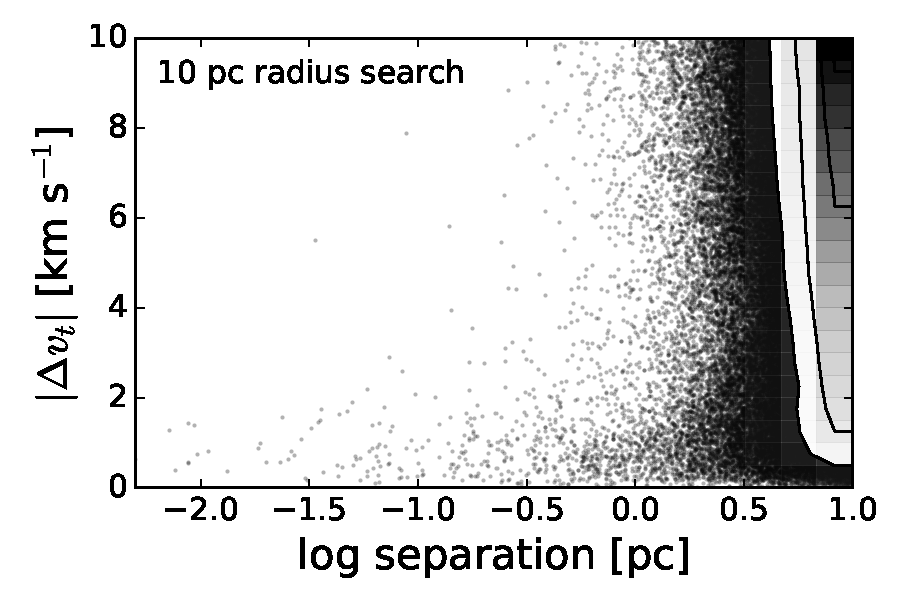
\includegraphics[width=\textwidth]{figures/sep_dvtan.pdf}
  \end{center}
  \caption{%
    Point estimates of tangential velocity and physical separation computed for
    all 271,232 unique pairs in the initial sample of pairs (black points).
    For this sample, we consider stars
    with separation $< 10$~pc and $\absdvtan < 10$~\kms\
    computed relative to every other star in \tgas.
    The blue solid line shows the magnitude of the 3D
    orbital velocity as a function of semi-major axis for a $2~M_\odot$ binary system.
    Note the stream of points that starts at small separation ($\lesssim 0.01$~pc),
    small $\absdvtan$ ($\lesssim 2$~\kms),
    but climbs to larger $\absdvtan$ at $|\Delta \vec{x}|\gtrsim 1$~pc, which
    eventually merges with random pairs of field stars dominating in the upper right corner
    (see \sectionname~\ref{sec:data} for details).
    \label{fig:dv-sep}}
\end{figure*}

\section{Methods} \label{sec:methods}

The abundance of pairs of stars with small velocity difference in
\figname~\ref{fig:dv-sep} suggests that there are a
significant number of co-moving stars in the \tgas\ data at a range
of separations.
Here we develop a method to select high-confidence co-moving
stars that properly incorporates the complex uncertainties associated with the
\gaia\ data. We make the following assumptions in order to construct a
statistical model (a likelihood function with explicit priors on our
parameters):
\begin{itemize}
  \item We assume that the uncertainties in the data---parallax, $\varpi$, and
    two proper motion components, $\propm = (\begin{array}[t]{c c} \mu_\alpha &
    \mu_\delta\end{array})^\mathsf{T}$---are Gaussian with known covariances
    $\mat{C}$. The values of covariances are provided by the \gaia\ data
    \citep{Lindegren:2012aa,Lindegren:2016aa}.
  \item We assume that the 3-space velocities of a given pair of stars
    $(\vec{v}_i, \vec{v}_j)$ in the \tgas\ sample (relative to the solar system
    barycenter) are either (1) co-moving with velocity drawn from a velocity
    prior $p(\vec{v})$ and  velocity difference drawn from a zero-mean Gaussian
    with velocity dispersion $s$, or (2) individually drawn from the same
    velocity prior $p(\vec{v})$.
\end{itemize}

Under these assumptions, the likelihood of a proper motion measurement,
$\bs{\mu}$, for a star given true distance, $d$, and true tangential velocity,
$\vec{v}^\perp =
(\begin{array}[t]{c c} v_\alpha & v_\delta\end{array})^\mathsf{T}$ is
\begin{align}
  L(\vec{v}, d, s^2) &=
    \left[\det\left(\frac{\tilde{\mat{C}}^{-1}}{2\pi}\right)\right]^{1/2} \,
    \exp \left[ -\frac{1}{2} \transp{\left(\vec{\mu} - \vec{x}_\theta \right)} \,
    \tilde{\mat{C}}^{-1} \,
    \left(\vec{\mu} - \vec{x}_\theta \right) \right] \label{eq:likefn} \\
  \vec{x}_\theta &= d^{-1} \, \vec{v}^\perp
\end{align}
where the tangential velocity $\vec{v}^\perp$ is related to the 3-space velocity
$\vec{v}$ through projection onto a tangent plane at a given star's sky position
$(\alpha, \delta)$
\begin{align}
  \vec{v}^\perp &= \mat{M}\,\vec{v} \\
  & = \left(
      \begin{array}{c c c}
        -\sin\alpha & \cos\alpha & 0 \\
        -\sin\delta \, \cos\alpha & -\sin\delta \, \sin\alpha & \cos\delta
      \end{array}
    \right) \,
    \left(\begin{array}{c} v_x \\ v_y \\ v_z \end{array}\right) \label{eq:transformation}
\end{align}
and the modified covariance matrix $\tilde{\mat{C}}$ is
\begin{equation}
  \tilde{\mat{C}} = \mat{C} + s^2 \, \eye
\end{equation}

We compute the fully marginalized likelihood (FML) that a given pair of stars
has the same 3-space velocity with a small velocity difference drawn from a
zero-mean Gaussian with variance $s^2$ (hypothesis 1, $\mathcal{L}_1$), and
the FML of the stars having independent 3-space velocities (hypothesis 2,
$\mathcal{L}_2$).
We use the FML ratio $\mathcal{L}_1/\mathcal{L}_2$ as a scalar for selecting
candidate co-moving stars, as described in $\sectionname~\ref{sub:selection}$ in
more detail.
To compute these FMLs, the likelihood functions for each star in a pair, $L_i,
L_j$, are marginalized over true 3-space velocity and distance for each star in
the pair $(i,j)$.
\begin{align}
  \mathcal{L}_1 &=
    \int \, \dd d_i \, \dd d_j \, \dd^3 \vec{v} \,
    L_i(\vec{v}, d_i, s^2) \,
    L_j(\vec{v}, d_j, s^2) \,
    p(\vec{v}) \, p(d_i \given \varpi_i) \, p(d_j \given \varpi_j) \\
  \mathcal{L}_2 &=
    \int \, \dd d_i \, \dd d_j \, \dd^3 \vec{v}_i \, \dd^3 \vec{v}_j \,
    L_i(\vec{v}_i, d_i, 0) \,
    L_j(\vec{v}_j, d_j, 0) \,
    p(\vec{v}_i) \, p(\vec{v}_j) \, p(d_i \given \varpi_i) \, p(d_j \given \varpi_j). \label{eq:hyp2}
\end{align}
The marginalization integral for hypothesis 2 can be split into the product of
two simpler integrals $\mathcal{L}_2 = Q_i \, Q_j$ where
\begin{equation}
  Q = \int \, \dd d \, \dd^3 \vec{v} \, L(\vec{v}, d, 0) \, p(\vec{v}) \, p(d\given\varpi)
\end{equation}
If the velocity prior $p(\vec{v})$ is also Gaussian, the integrals over velocity
in both cases can be performed analytically:
We use a mixture of three isotropic, zero-mean Gaussian distributions
\begin{equation}
  p(\vec{v}) = \sum_{m=1}^3 \, w_m \mathcal{N}(0, \sigma_{v,m}^2)
\end{equation}
with velocity dispersions $(\sigma_{v,1}, \sigma_{v,2}, \sigma_{v,3}) = (15, 30, 50)
~\kms$ and weights $(w_1,w_2,w_3) = (0.3, 0.55, 0.15)$
meant to encompass young thin disk stars to halo stars.
We derive the relevant expressions in Appendix~\ref{sec:appendix}.
After marginalizing over velocity, the likelihood integrands only depend on
distance; we numerically compute the integrals over the true distances to each
star in a pair, $d_1,d_2$, using Monte Carlo integration with $K$ samples from
the distance posterior pdfs \todo{Comment on the choice of distance prior}:
\begin{equation}
  \int \, \dd d \, \tilde{L}(d) \, p(d\given\varpi) \approx
    \frac{1}{K} \, \sum_k^K \, \tilde{L}(d_k)
\end{equation}
where $\tilde{L}(d)$ is the velocity-marginalized likelihood function.
Through experimentation, we have found that $K=128$ samples are sufficient for
estimating the above integrals for stars with a wide range in parallax
signal-to-noise.
%TODO: SMOH: still unsure about this

For wide binaries, the assumption of the stars having the same 3D velocity can
break down for high precision proper motion measurements because of the orbital
velocity (blue solid line in Figure~\ref{fig:dv-sep}).
To account for this, we set $s^2 = \frac{2 \, G \, \msun}{|\vec{x}_i-\vec{x}_j|}$.

\section{Results} \label{sec:results}

This section is divided into three parts. First, we discuss and justify a cut of
the likelihood ratio to select candidate co-moving pairs.
Second, we present the statistics and properties of our candidate co-moving
pairs.
Finally, we describe our catalog of candidate co-moving pairs, the main product
of this study.

\subsection{Selecting candidate co-moving pairs}
\label{sub:selection}

In this section, we examine the distribution of (log-)likelihood ratios
$\ln \mathcal{L}_1 /\mathcal{L}_2$, and come up with a reasonable cut
for this quantity to select co-moving pairs from the initial pairs sample.

\begin{figure*}[htbp]
  \begin{center}
    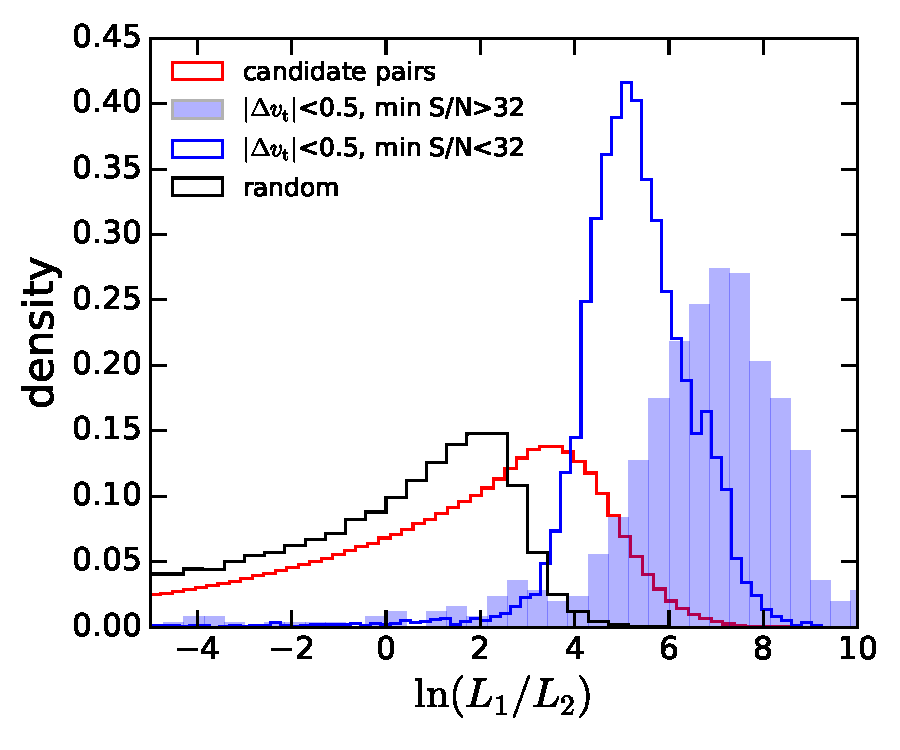
\includegraphics[width=\textwidth]{figures/likelihoodratios.pdf}
  \end{center}
  \caption{%
    Left: Density histogram of likelihood ratios for candidate pairs and random pairs.
    Along with the distribution for the entire candidate pairs (black thick line),
    we show the distribution for subsets in slices of $\Delta v_t$.
    Right: $\Delta v_t$ vs separation in slices of $\ln \mathcal{L}_1 /\mathcal{L}_2$.
    \label{fig:likelihoodratios}}
    \vspace{1em}
\end{figure*}

Figure~\ref{fig:likelihoodratios} shows the likelihood ratios for all
$\approx$271k initial pairs examined.
As discussed in \sectionname~\ref{sec:data}, we expect a correlation between likelihood
ratios of pairs, and their distribution in $\Delta v_t$ vs separation plane.
Specifically, as we sweep through from small $\Delta v_t$ to large, we expect
the population of pairs to change from genuinely co-moving to random.
This becomes clear when we look at the distribution of likelihood ratios for
slices of $\Delta v_t$ centered at 0.5, 5, and 9.5~\kms.
\todo{Fix in below and in the figure, $\Delta v_t$ should be $|\Delta v_t|$}
Pairs with $|\Delta v_t-0.5|<0.5$ are most likely actual co-moving pairs, and
their likelihood distribution is narrowly peaked above 6.
The distribution peaks at lower values and gets broader as $\Delta v_t$ increases,
and the number of random pairs increasingly dominate.
On the right panel of Figure~\ref{fig:likelihoodratios}, we show
how the distribution of pairs on $\Delta v_t$ vs separation plane changes
with decreasing $\ln \mathcal{L}_1 /\mathcal{L}_2$ ratios.
This is in agreement with our discussion in \sectionname~\ref{sec:data}.
Finally, as a test,
we compute the likelihood ratios for 200,000 random pairs of stars with the same
parallax signal-to-noise ratio cut as candidate pairs ($S/N > 8$).
Shown as gray shaded histogram in Figure~\ref{fig:likelihoodratios},
this distribution peaks at a much lower value ($\approx 2$),
and is clearly separated from highly probable co-moving pairs.

Based on these comparisons, we select pairs with
$\ln \mathcal{L}_1 /\mathcal{L}_2 > 6$ as co-moving pair candidates.
Out of 271,232 candidate pairs examined, 13,058 pairs (4.8\%)
satisfy this condition.

\subsection{Statistics, properties, and nature of co-moving pairs}

\begin{figure*}[htbp]
  \begin{center}
    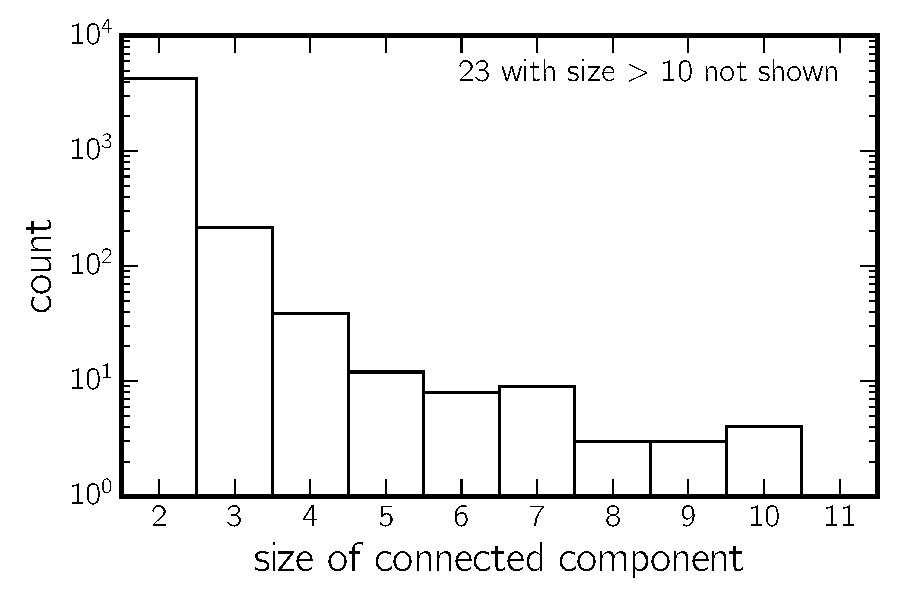
\includegraphics[width=\textwidth]{figures/dist_networksize.pdf}
  \end{center}
  \caption{%
    Histogram of the sizes of connected components.
    \label{fig:hist_ccsize}}
\end{figure*}

\begin{figure*}[htbp]
  \begin{center}
    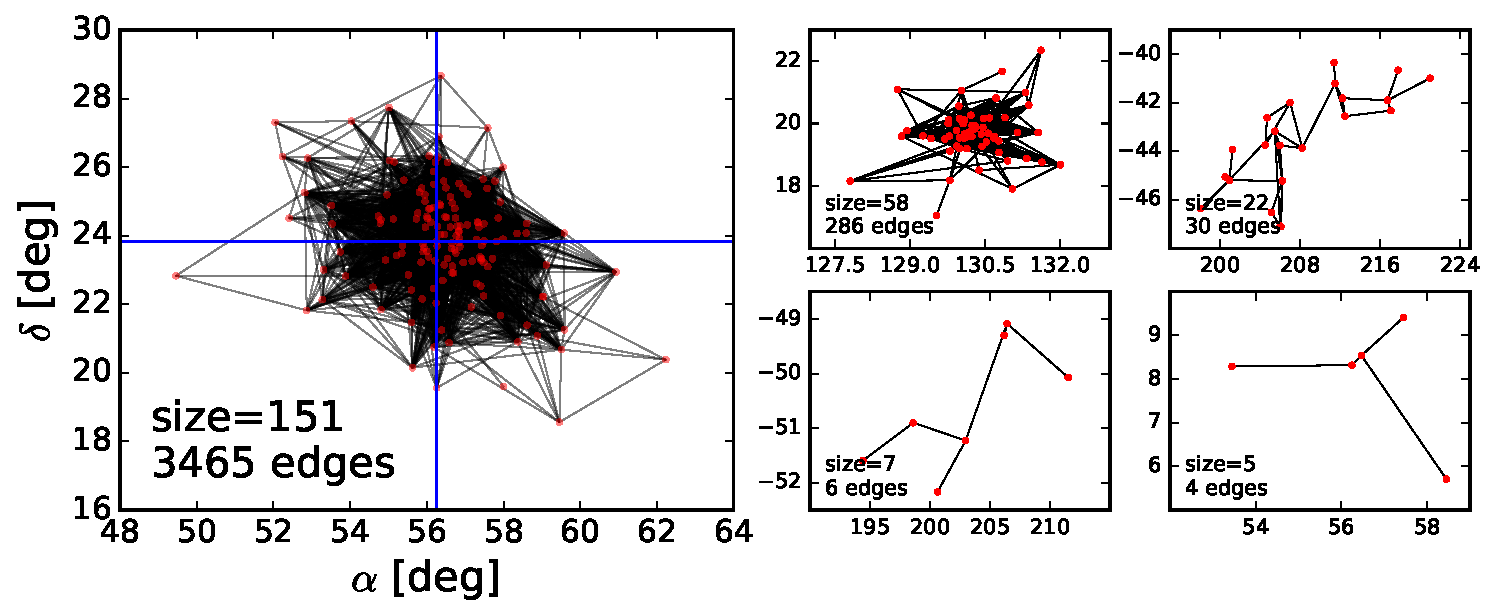
\includegraphics[width=\textwidth]{figures/graphviz_examples.pdf}
  \end{center}
  \caption{%
    Visualizations of a few example connected components of co-moving pairs of stars.
    Each star (node) is marked as a red circle, and a line (edge) is drawn
    between two stars if they are co-moving by our selection criteria
    (see \sectionname~\ref{sub:selection}). On left, we show the largest network
    found in this study corresponding to the Pleiades star cluster.
    On right, we show four examples of connected components with varying sizes.
    The connected component on the upper left panel with a size of 58 corresponds
    to NGC~2632, also known as the Beehive cluster.
    \label{fig:graphviz_examples}}
\end{figure*}

\begin{figure*}[htbp]
  \begin{center}
    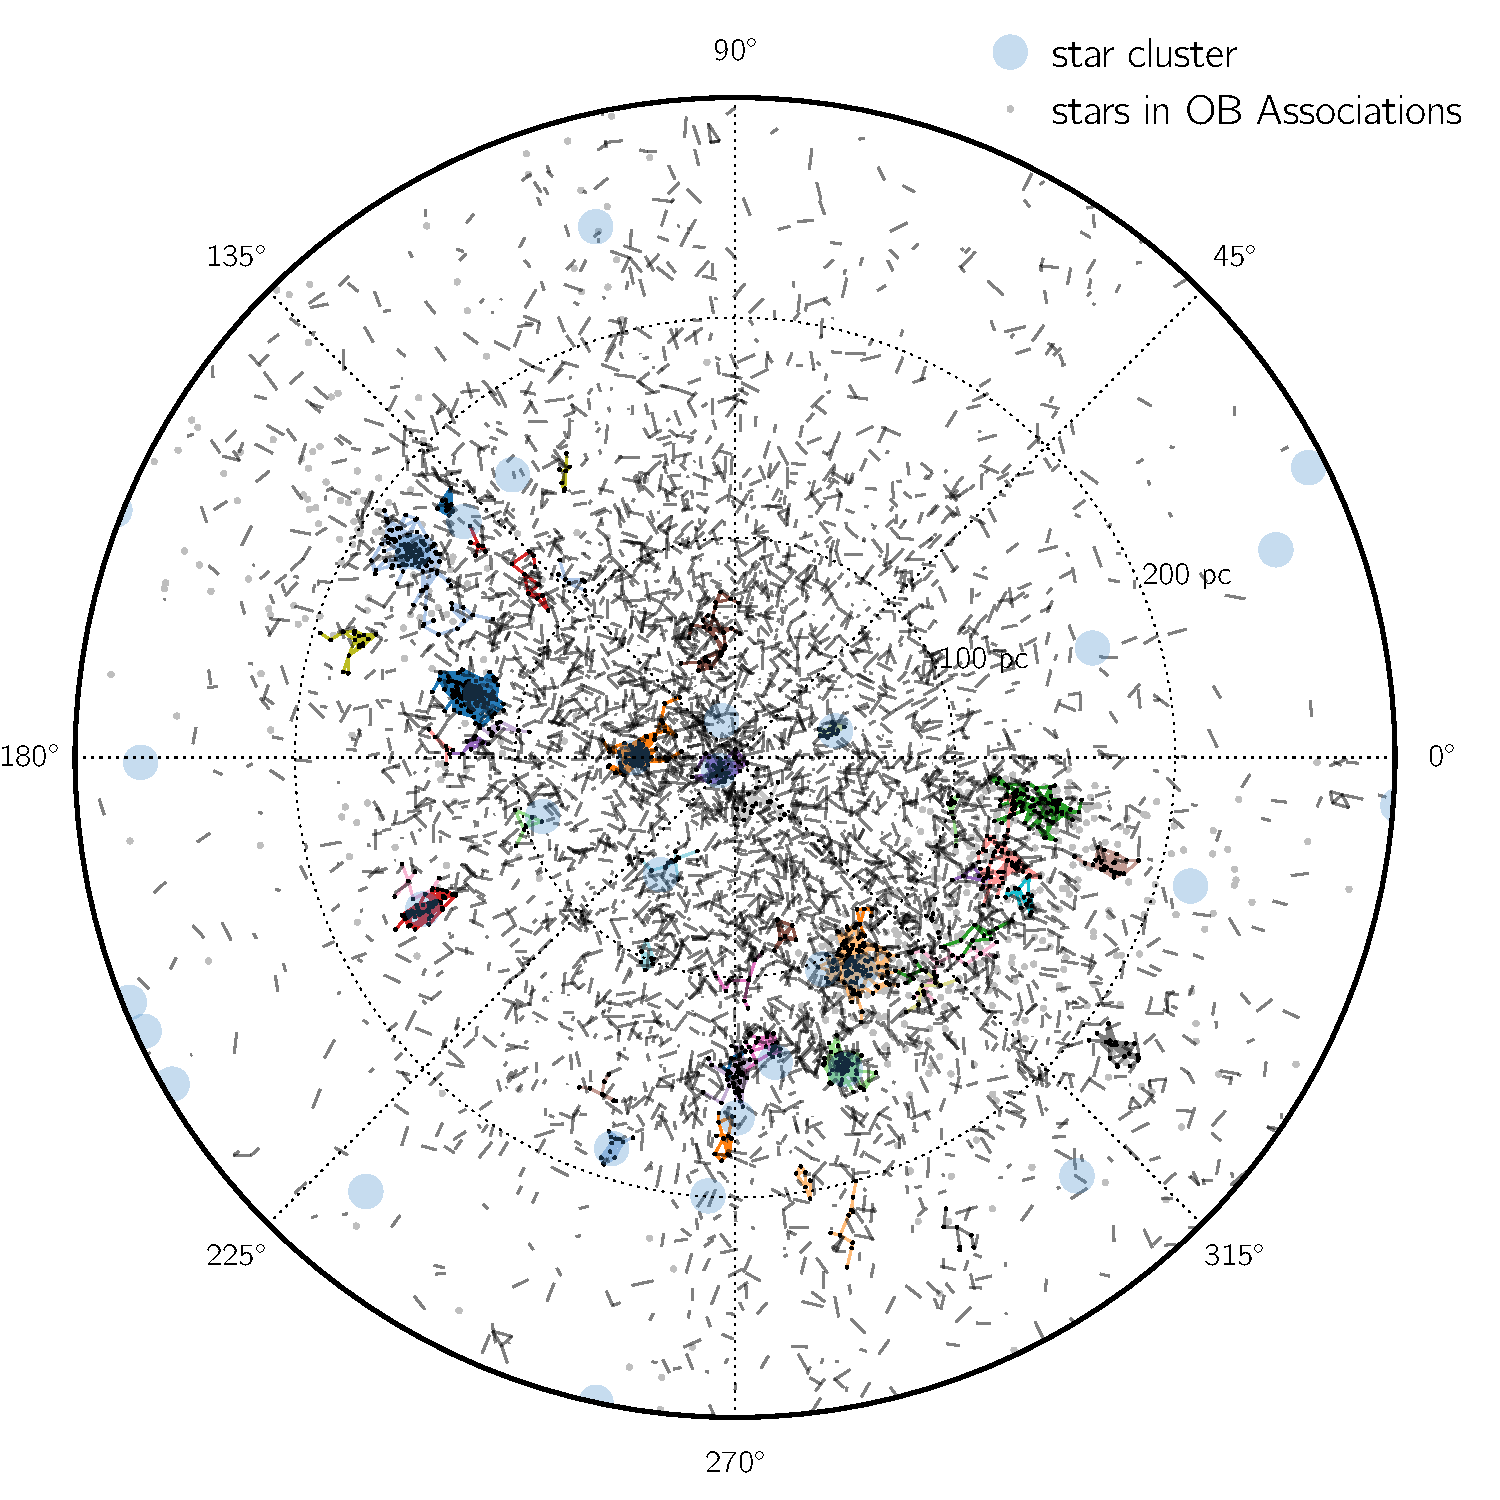
\includegraphics[width=\textwidth]{figures/glon_d_pie.pdf}
  \end{center}
  \caption{%
    Panoramic view of co-moving pairs of stars. This is a cylindrical
    projection of onto the Galactic plane. The angle is the Galactic
    longitude, and the radius is $d\cos b$ in pc where $d$ is the point-estimate
    of distance using Equation~\ref{eq:dist}.
    Pairs in connected components of sizes less than 5 are connected by gray lines.
    Pair in connected components of size $\geq 5$ are plotted with a unique color per network,
    and their nodes (stars) are highlighted with small black circles.
    We also show the positions of known Milky Way star clusters
    from \citet{Kharchenko:2016aa} as empty purple circles,
    and stars in OB associations from \citet{de-Zeeuw:1999aa} as
    gray circles.
    \label{fig:glon_d_pairlines}}
\end{figure*}

Once we have identified candidate co-moving star pairs from the initial pair
sample, these pairs form an undirected graph where stars are nodes, and edges
between the nodes exist for co-moving pairs of stars.
A star may have multiple co-moving neighbors, and two stars may either
be directly or indirectly connected by a set of edges.
We divide the network into connected components\footnote{A connected component of an undirected graph $G$
is a subgraph of $G$ in which any two nodes are connected to each other by a path.
We use the term ``network'' loosely to refer to a graph or its connected components.},
and show the distribution of their sizes in Figure~\ref{fig:hist_ccsize}.
The most common are size 2 networks, which mean mutually exclusive co-moving
pairs. However, it is clear that there are many aggregates of co-moving stars
discovered by looking for co-moving pairs.
These aggregates are likely moving groups, OB associations, or star clusters.
There are 4555 connected components among 10,606 unique stars.
The maximum size of connected components is 151.
We show this largest network along with four randomly selected
examples of networks with sizes greater than 4 in Figure~\ref{fig:graphviz_examples}.
The largest network corresponds to the Pleiades open cluster.
One particular star in this network, TYC 1799-272-1, has 94 directly connected
co-moving neighbors, and is located at the center of the network.

We show the distribution co-moving pairs in galactic longitude and
distance in Figure~\ref{fig:glon_d_pairlines}.
The connection between known co-moving structures and the networks of co-moving
pairs found in this work becomes immediately clear when
we overplot the positions of known Milky Way star clusters \citep{Kharchenko:2016aa},
and stars in OB associations \citep{de-Zeeuw:1999aa}.
Many of the larger networks are clearly associated with known star clusters.
The most prominent is Melotte 111 at
$(l,d)\approx (220\arcdeg, 87~\textrm{pc})$ otherwise known as the Coma star cluster.
Clumps of co-moving pairs at $(l,d)\approx (300-360\arcdeg, 100-200~\textrm{pc})$
seem to strongly correlate with the locations of OB associations
Upper Scorpius, Upper Centaurus Lupus, and Lower Centaurus Crux
\citep{de-Zeeuw:1999aa}.

Ultimately, any candidate co-moving pair found in this work
needs to be verified using radial velocities.
Here, we use 210,368 cross-matches of \tgas\ with
the Radial Velocity Experiment (\rave) to
assess the false positive rates of our selection.
We have 283 pairs with both stars matched with \rave.
Figure~\ref{fig:raverv} shows the difference in radial velocities
between the two stars in a pair, $\Delta v_r$, as a function of their physical separation.
We show $\Delta v_r$ in units of $\sigma_{\Delta v_r}$ which we estimate
as the quadrature sum of $\sigma _{v_r}$ for each star.
The fraction of pairs with good agreement in radial velocity decreases with
increasing separation.
This, after all, is not surprising because we are only using
2D velocity information (proper motions) with errors.
However, the contamination becomes significant only at $>1$~pc
(which depends on the local stellar number density and velocity dispersion).
Given the excellent correspondence between co-moving pair networks of larger sizes
and known genuine co-moving structures (Figure~\ref{fig:glon_d_pairlines}),
we may expect that pairs in these larger networks which will often have
separations $>1$~pc to have less contamination.
We divide pairs into those mutually exclusively connected (i.e., in a network of
size 2), and those in a larger network.
We indeed find that many pairs in larger networks are at $>1$~pc, yet
the fraction of pairs that have identical radial velocities within $3\sigma$ is
higher than mutually exclusive pairs, and remains high ($>80\%$) to $\sim 10$~pc.

\begin{figure}[htbp]
  \begin{center}
    % 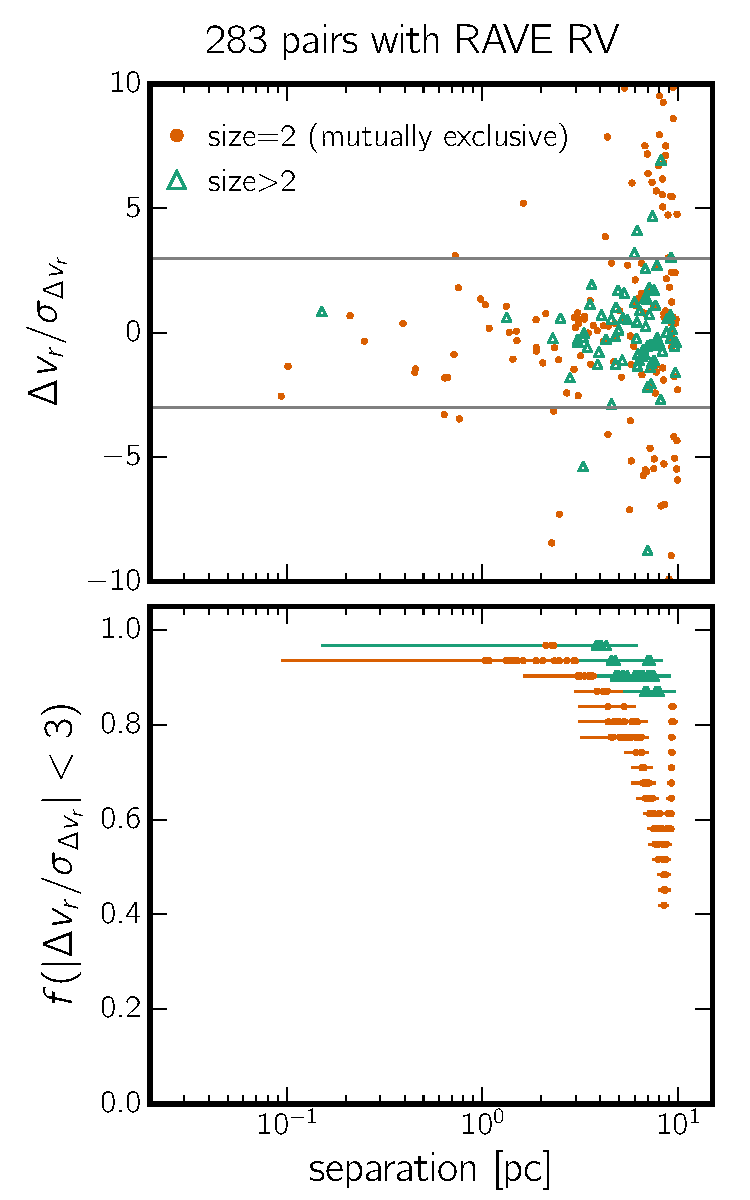
\includegraphics[width=\linewidth]{figures/raverv.pdf}
    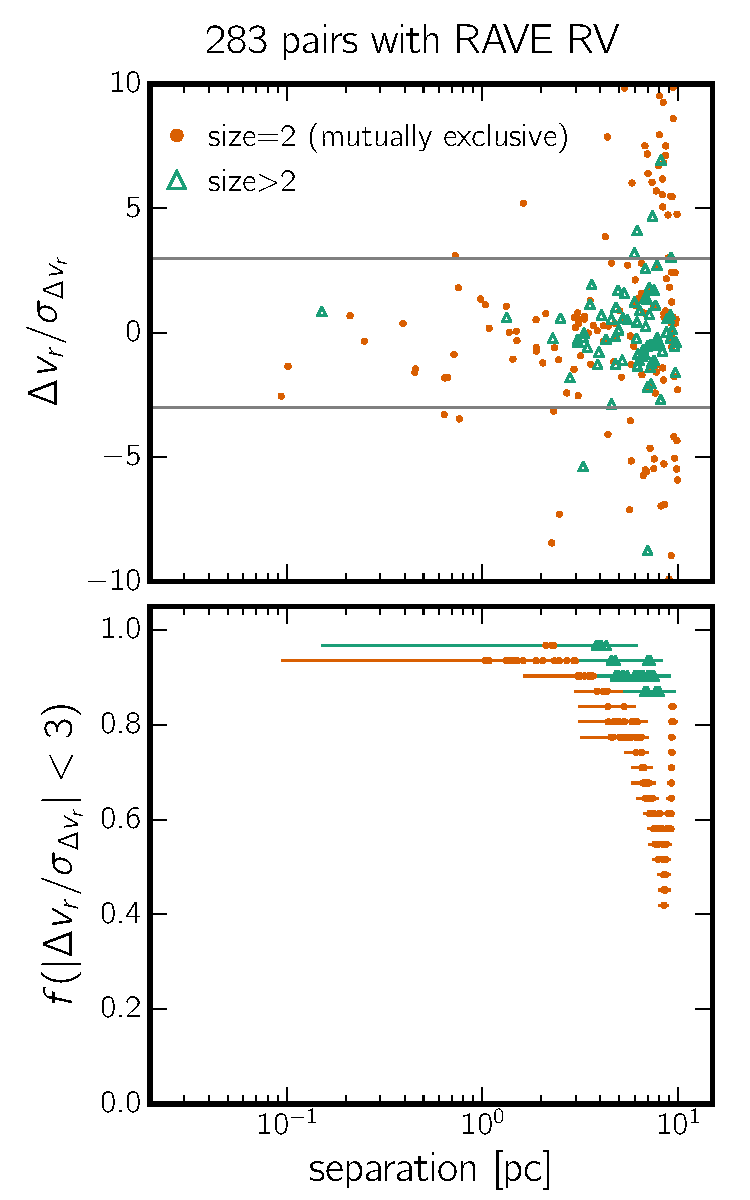
\includegraphics[width=.5\linewidth]{figures/raverv.pdf}
  \end{center}
  \caption{%
    Validation of candidate co-moving pairs using radial velocities from \rave.
    Top: Radial velocity differences, $\Delta v_r$, of 283 pairs with \rave\ measurements.
    $\Delta v_r$ is plotted in units of $\sigma_{\Delta v_r} = \sqrt{\sigma_{v_r,1}^2 + \sigma_{v_r,2}^2}$
    as a function of physical separation.
    We highlight $3\sigma$ limit with two horizontal lines.
    Bottom: Fraction of pairs with $\Delta v_r/\sigma_{\Delta v_r} <3$
    as a function of physical separation. We calculate the fraction with a running
    bin containing 31 data points at a time.
    The median, and the minimum and maximum separation of pairs in each bin are
    indicated with a marker, and its errorbars.
    We separate pairs in connected components of size 2 (i.e., mutually exclusively connected)
    from those in larger connected components.
    \label{fig:raverv}}
\end{figure}

We now examine the separation distribution of co-moving pairs in
Figure~\ref{fig:hist_separation}.
As expected, pairs in larger networks are mostly found with separations
larger than 1~pc.
Surprisingly, however, we also find a huge number of mutually exclusive pairs
at $>1$~pc as well. Even if we consider the increasing false positive rate at large
separations, the distribution is not significantly changed as the number of pairs
at $>1$~pc is in fact increasing much faster (as a power-law)
than the decrease due to the false positives (right panel of Figure~\ref{fig:raverv}).
The nature of these very large separation, mutually exclusive pairs,
which cannot be gravitationally bound to each other, needs further investigation.
Can they be remnants of escaped binaries that are drifting apart?
In a study of the evolution of wide binaries including the Galactic tidal field
as well as passing field stars, \citet{Jiang:2010aa} found that we expect
to find a peak at $\sim 100-300$~pc in the projected separation due to
stars that were once in a wide binary system, but are drifting apart with small
relative velocities ($\sim 0.1$~\kms).
Our search which stops on the maximum radius of 10~pc is obviously insufficient
to clearly detect this peak, but it shows such hint, and demonstrates
that such large scale phase-space correlations may now be looked for and studied within the \gaia\ data.

\begin{figure*}[htbp]
  \begin{center}
    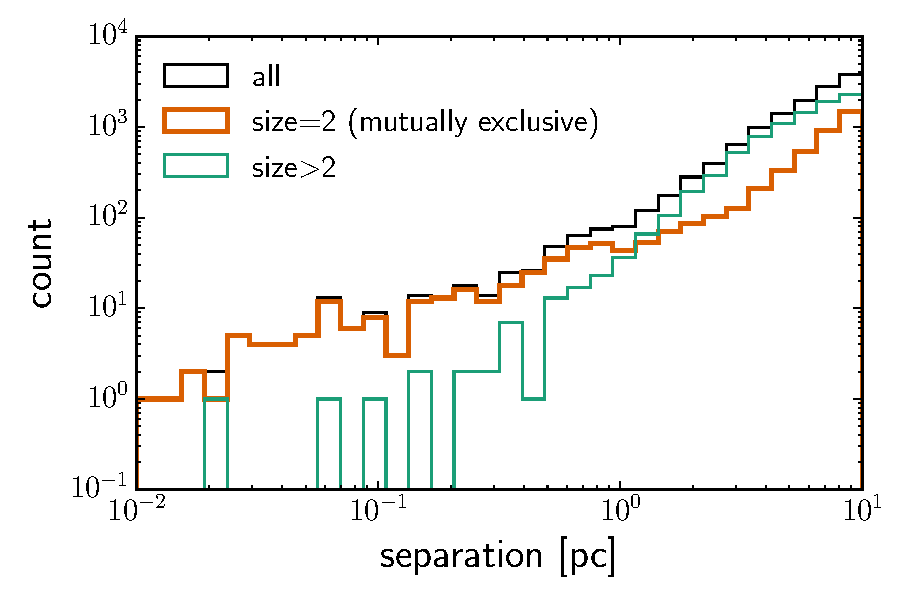
\includegraphics[width=\textwidth]{figures/hist_sep.pdf}
  \end{center}
  \caption{%
    Separation distribution of co-moving pairs of stars.
    As with Figure~\ref{fig:raverv},
    we divide the pairs into those mutually exclusively connected
    (connected component size $=2$), and those connected to larger connected components (size $>2$).
    \label{fig:hist_separation}
    }
\end{figure*}

Finally, we present the color-magnitude diagrams of co-moving pairs
using the cross-matches with \tmass.
A more detailed study of stellar parameters using photometry from various sources
will follow. Figure~\ref{fig:cmd_large} and \ref{fig:cmd_me} shows $G-J$ vs $G$
color-magnitude diagrams for stars in larger networks (size$>2$) and in mutually
exclusive pairs (networks of size 2), respectively.
The networks shown in Figure~\ref{fig:cmd_large} correspond to those visualized
in Figure~\ref{fig:graphviz_examples}.
For stars in larger networks, there is a noticeable lack of evolved, off-main sequence
stars, in agreement with these kinematic structures being young.
For mutually exclusive pairs, we divide the pairs by separation at 1~pc
above which the false positive rate due to random pairs starts to increase.
While many pairs are located along the main sequence, we also find
quite a few of main sequence-red giant pairs,
which will be valuable to anchoring stellar atmospheric models together.
%TODO: SMOH: what else can i discuss?

\begin{figure*}[htbp]
  \begin{center}
    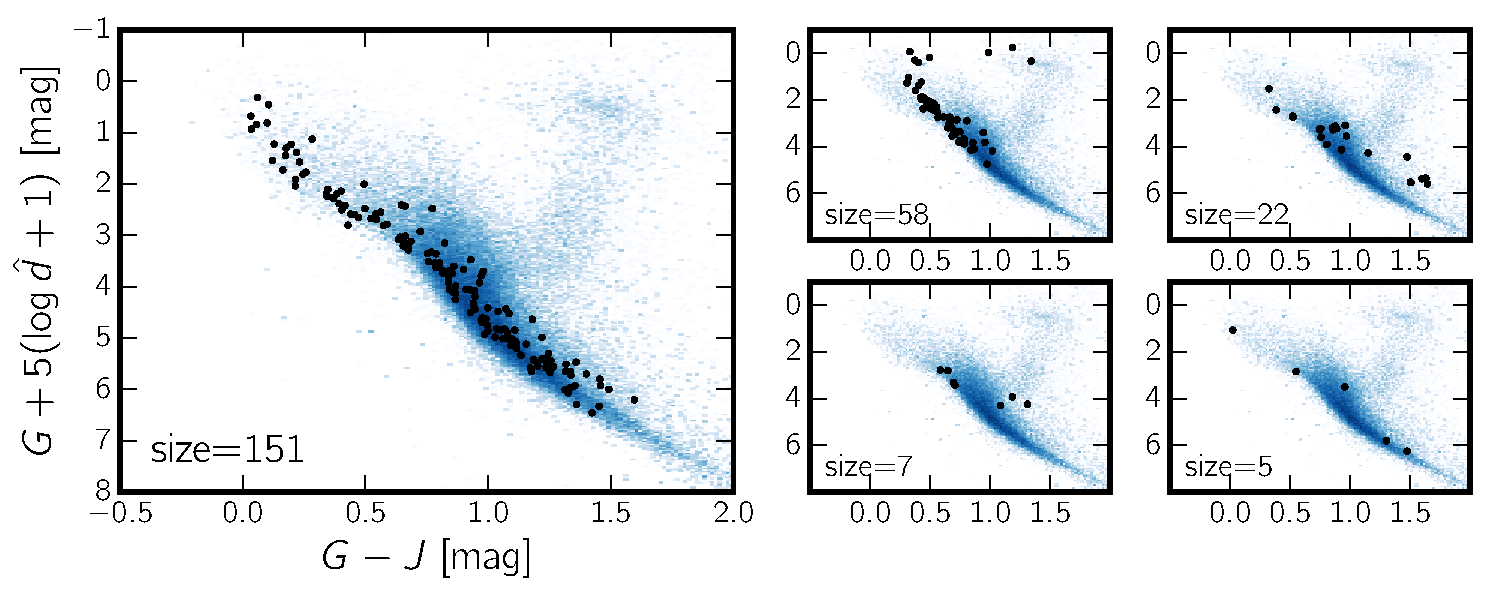
\includegraphics[width=\textwidth]{figures/gjg_graphviz_examples.pdf}
  \end{center}
  \caption{
    Color-magnitude diagrams of stars in larger networks presented in
    Figure~\ref{fig:graphviz_examples}. Each panel shows the same network
    visualized in the panel at the same position
    in Figure~\ref{fig:graphviz_examples}.
    We show the distribution of all stars common in \tgas\ and \tmass\
    with parallax $S/N>16$ in blue for reference.
    \label{fig:cmd_large}}
\end{figure*}

\begin{figure*}[htbp]
  \begin{center}
    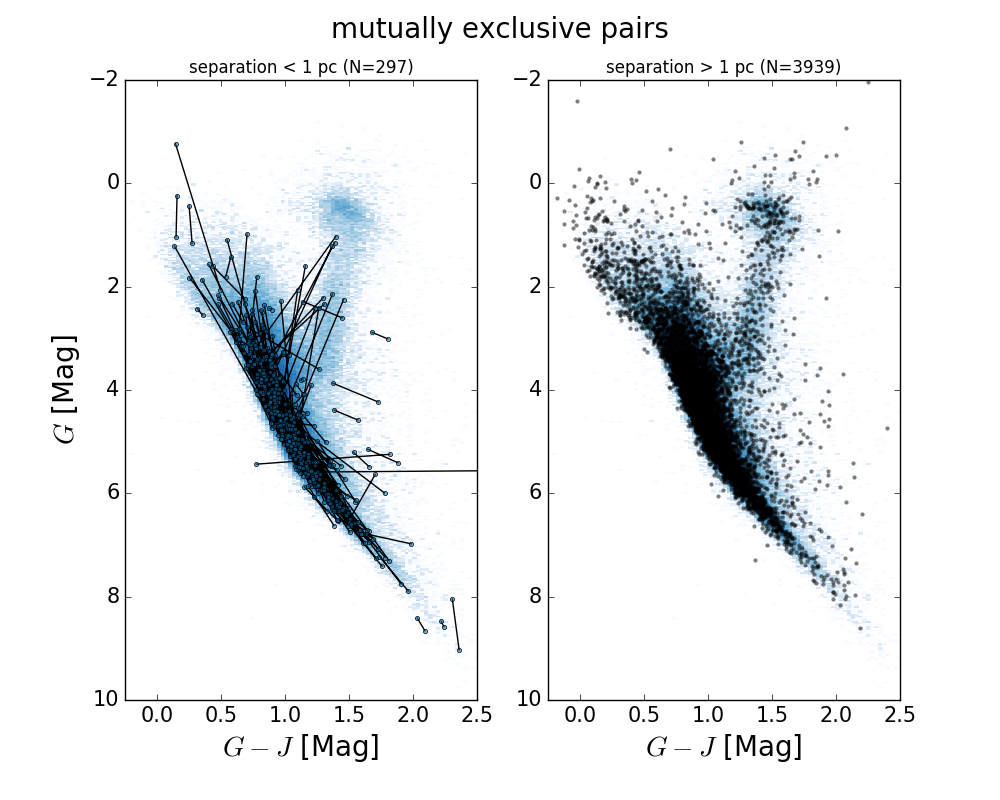
\includegraphics[width=\textwidth]{figures/gjg_mepairs.png}
  \end{center}
  \caption{
    Color-magnitude diagrams of stars in networks of size 2 (i.e., mutually exclusive)
    in two separation bins.
    We connect each pair by a line on the left for pairs with separations smaller than
    1~pc.
    We show the distribution of all stars common in \tgas\ and \tmass\
    with parallax $S/N>16$ in blue for reference same as in Figure~\ref{fig:cmd_large}.
    \label{fig:cmd_me}}
\end{figure*}

\subsection{Catalog of candidate co-moving pairs}

In this section, we describe our catalog of candidate co-moving pairs of stars.
For 13,058 pairs (10,606 unique stars) found in this work,
we provide the following information:
%
\begin{itemize}
  \item \tgas\ source id for the two stars in a pair; these may be used to easily
  retrieve cross matches of \gaia\ with other surveys such as WISE, \tmass, and \rave
  using the \gaia\ data archive.
  \item physical separation between the two stars in pc
  \item likelihood ratio, $\ln \mathcal{L}_1 /\mathcal{L}_2$
  \item size of the network that the pair belongs to
  \item unique ID of the network that the pair belongs to
\end{itemize}
%
Additionally, given the strong correlation between the larger networks of pairs
and the known star clusters and OB associations, we provide for each star
%
\begin{itemize}
  \item index of the closest cluster in the Milky Way Star Cluster catalog of
  \citet{Kharchenko:2016aa} using 3D separation
  \item distance to the closest cluster in pc
  \item the ID of the OB association (A-L) if the star is in the catalog of
  stars in the known OB associations by \citet{de-Zeeuw:1999aa}
\end{itemize}
%
A part of the entire table is presented in Table~\ref{tab:catalog}.

\begin{deluxetable*}{cccccc}
\tablecaption{Catalog of candidate co-moving pairs \label{tab:catalog}}
\tablehead{\colhead{star1 source id} & \colhead{star2 source id} & \colhead{separation} & \colhead{$\ln \mathcal{L}_1 /\mathcal{L}_2$} & \colhead{ID$_\mathrm{CC}$} & \colhead{$N_\mathrm{CC}$}\\ \colhead{ } & \colhead{ } & \colhead{$\mathrm{pc}$} & \colhead{ } & \colhead{ } & \colhead{ }}
\startdata
249282341403694592 & 441371523899475840 & 4.9 & 7.0 & 1 & 125 \\
249087281167662464 & 441901694662492928 & 8.3 & 7.1 & 1 & 125 \\
64933755122821120 & 66786500935624320 & 7.8 & 7.5 & 0 & 151 \\
436536249718223744 & 441356921010671232 & 6.5 & 6.5 & 1 & 125 \\
3953625835302703488 & 4008706729289355520 & 6.1 & 6.3 & 8 & 47 \\
63730305286697600 & 65188085906203520 & 7.0 & 6.6 & 0 & 151 \\
1873311936758998016 & 1873312074197947392 & 7.5 & 7.2 & 4013 & 2 \\
5814505765886192512 & 5814997419380722944 & 6.1 & 6.2 & 14 & 20 \\
350903157411208832 & 352510643410053632 & 9.9 & 6.8 & 565 & 2 \\
64114241002810496 & 67618281484716544 & 7.2 & 6.1 & 0 & 151
\enddata
\tablecomments{Table 1 is published in its entirety in the machine-readable format. A portion is shown here for guidance regarding its form and content.}
\end{deluxetable*}


We note a caveat on the completeness of the networks found in our catalog.
Because we applied a simple cut in the likelihood ratio ($\ln \mathcal{L}_1 /\mathcal{L}_2>6$),
there is a possibility that, for example, a star in a mutually exclusive pair in our catalog may
still have another possibly co-moving companion which has been dropped because the likelihood ratio
is slightly less than 6.

\section{Conclusions}\label{sec:conclusions}

In this \documentname, we looked for co-moving pairs of stars in the
\tgas\ data released as part of the \gaia\ DR1.
Our method is to compare
the fully marginalized likelihoods between the two hypotheses, that a pair of
stars shares the same 3D velocity, and that the two stars have two independent
3D velocities, incorporating the errors in parallax and proper motions.
We argued for a reasonable cut of the likelihood ratio, and found
13,058 candidate pairs of co-moving stars among 10,606 unique stars
with separation ranging from 0.005~pc to 10~pc, the limit of our search.

We examined the network of co-moving stars, and found that many of the larger
networks of co-moving stars naturally corresponds to some of the known co-moving structures
such as open clusters and stellar associations.
We have also found a surprisingly large number of very wide separation ($>3$~pc)
co-moving pairs which are not clearly associated to any known existing clusters.
While their nature is yet unclear, they may be remnants of dissolving wide binaries and
open clusters. If so, this population should still be relatively young compared
to the general disk field population. Modeling the color-magnitude diagram
distribution of these stars can shed some light on this issue.
If they are truly dissolving stars that were born coeval,
the sample of very wide separation co-moving pairs can potentially be used
to measure the recent ($\lesssim 1$~Gyr)
star formation history in the Solar neighborhood.
Co-moving stars with separation less than 1~pc are very promising candidates
for wide binaries. They are found to be pairs of stars of varying stellar types.
Some of these pairs, such as main sequence-red giant or FGK-M dwarfs,
will be particularly valuable for testing theoretical
stellar models and calibrating observational measurements of low mass stars.


\acknowledgements

This work has made use of data from the European Space Agency (ESA)
mission {\it Gaia} (\url{http://www.cosmos.esa.int/gaia}), processed by
the {\it Gaia} Data Processing and Analysis Consortium (DPAC,
\url{http://www.cosmos.esa.int/web/gaia/dpac/consortium}). Funding
for the DPAC has been provided by national institutions, in particular
the institutions participating in the {\it Gaia} Multilateral Agreement.
This project was developed in part at the 2016 NYC Gaia Sprint,
hosted by the Center for Computational Astrophysics at the Simons Foundation in New York City.

This research was partially supported by the \acronym{NSF} (grants
  \acronym{IIS-1124794}, \acronym{AST-1312863}, \acronym{AST-1517237}),
  \acronym{NASA} (grant \acronym{NNX12AI50G}),
  and the Moore-Sloan Data Science Environment at \acronym{NYU}. The data
analysis presented in this article was partially performed on computational
resources supported by the Princeton Institute for Computational Science and
Engineering (PICSciE) and the Office of Information Technology's High
Performance Computing Center and Visualization Laboratory at Princeton
University.


\software{The code used in this project is available from
\url{https://github.com/smoh/gaia-wide-binaries} under the MIT open-source
software license. This version was generated at git commit
\texttt{\githash\,(\gitdate)}.
This research additionally utilized:
    \texttt{Astropy} (\citealt{Astropy-Collaboration:2013}),
    %\texttt{emcee} (\citealt{Foreman-Mackey:2013}),
    \texttt{IPython} (\citealt{Perez:2007}),
    \texttt{matplotlib} (\citealt{Hunter:2007}),
    and \texttt{numpy} (\citealt{Van-der-Walt:2011}).}

% \facility{\sdssiii, \apogee}

\bibliographystyle{aasjournal}
\bibliography{refs}

\appendix

\section{Relevant properties of Gaussian integrals}
\label{sec:appendixA}

In what follows, all vectors are column vectors, unless we have transposed them.
A relevant exponential integral solution is
\begin{eqnarray}
  \ln\left[\int\exp(-\frac{1}{2}\,
    \transp{[\vec{x}-\vec{\nu}]} \,
    \inv{\mat{A}} \,
    [\vec{x}-\vec{\nu}] - \Delta) \, \dd \vec{x}\right]
  &=& +\frac{1}{2}\ln ||2\pi\,\mat{A}|| -\Delta
  \quad , \label{eq:gauss-int}
\end{eqnarray}
where $\vec{x}$ and $\vec{\nu}$ are $D$-dimensional vectors, $\mat{A}$ is a
positive definite matrix, $\Delta$ is a scalar, and the integral is over all of
$D$-dimensional $\vec{x}$-space.
To cast our problem in this form, we will need to complete the square of the
exponential argument.
If we equate
\begin{eqnarray}
  \frac{1}{2}\,\transp{[\vec{x}-\vec{\nu}]}\,\inv{\mat{A}}\,[\vec{x}-\vec{\nu}] + \Delta
  &=& \frac{1}{2}\,\transp{\vec{x}}\,\inv{\mat{A}}\,\vec{x} + \transp{\vec{x}}\,\mat{B}\,\vec{b} + C
  \quad ,
\end{eqnarray}
where $\mat{B}\,\vec{b}$ is an $D$-vector, and $C$ is a scalar, then we find
\begin{eqnarray}
  \vec{\nu} &=& -\mat{A}\,\mat{B}\,\vec{b}
  \\
  \Delta & = & C - \frac{1}{2}\,\transp{\vec{\nu}}\,\inv{\mat{A}}\,\vec{\nu}
  \quad .
\end{eqnarray}
We will identify terms in our likelihood functions with $\mat{A}$,
$\mat{B}\,\vec{b}$, and $C$, convert to $\vec{\nu}$ and $\Delta$ and compute
the marginalized likelihood using \eqname~\ref{eq:gauss-int}.

\section{Expressions for the marginalized likelihoods}\label{sec:appendix}

At given distance $d$, the velocity-marginalized likelihood can be computed
analytically using the expressions in Appendix~\ref{sec:appendixA}.
As described above, we use an isotropic, mixture-of-Gaussians prior on velocity
where the velocity dispersion of a given mixture component is $\sigma_{v,m}$ and
the 3-space variance tensor is $\mat{V}_m = \sigma_{v,m}^2 \, \eye$.
The likelihood for the data is also a Gaussian, as shown in
\eqname~\ref{eq:likefn}.
We will start by writing down expressions for the the likelihood multiplied by
the prior pdf for the velocities.
Here we slightly change the notation used in \sectionname~\ref{sec:methods} for
simplicity.

We construct a velocity-space data vector $y$ as follows:
\begin{equation}
  \vec{y} =
    \transp{\left(
      \begin{array}{c c c c}
        d_i\,\mu_{\alpha,i} &
        d_i\,\mu_{\delta,i} &
        d_j\,\mu_{\alpha,j} &
        d_j\,\mu_{\delta,j}
      \end{array}
    \right)}
\end{equation}
where again the subscripts $i,j$ refer to the indices of each star in the pair
and we have multiplied the observables (the proper motions) by the distances
$d_i, d_j$, which is permitted because we are conditioning on the distances.
Fundamentally, our hypothesis 1 model (the stars have the same velocity with a
small difference) is
\begin{equation}
  \vec{y} = \mat{M} \, \vec{v} + \mathrm{noise}
\end{equation}
where now the $4 \times 3$ transformation matrix $\mat{M}$ is a stack of the
transformation matrices for each star computed from the pair of sky positions
and using \eqname~\ref{eq:transformation}.
The noise (in the $y$ vector) is drawn from a $4 \times 4$ Gaussian with
block-diagonal covariance matrix, $\mat{\Sigma}$, constructed from the
covariance matrix of the observables, $\mat{C}_i, \mat{C}_j$, and the distances
$d_i, d_j$:
\begin{equation}
  \mat{\Sigma} = \left(
    \begin{array}{c c}
      d_i^2 \, \mat{C}_i & 0 \\
      0 & d_j^2 \, \mat{C}_j
    \end{array}
  \right)
\end{equation}

Given all these definitions, the likelihood function for hypothesis 1 is
\begin{eqnarray}
  p(\data \given \vec{v}, d_i, d_j) &=& d_i^2\,d_j^2\,
    \normal(\vec{y} \given \mat{M}\,\vec{v}, \mat{\Sigma}) \\
  \ln p(\data \given \vec{v}, d_i, d_j) &=& 2\,\ln d_i + 2\,\ln d_j
    -\frac{1}{2}\,\ln||2\pi\,\mat{\Sigma}|| \nonumber \\
    && \quad -\frac{1}{2}\,\transp{[\vec{y}-\mat{M}\,\vec{v}]}\,
      \inv{\mat{\Sigma}}\,
      [\vec{y}-\mat{M}\,\vec{v}]
  \quad ,
\end{eqnarray}
where the factor of $d_i^2\,d_j^2$ converts to units of one over \gaia\ data
from units of one over $y$, which includes the distances.

Now we multiply this likelihood with the velocity prior (here shown only for one
prior velocity mixture component) and complete the square.
In the original parameterization, we find:
\begin{eqnarray}
  \mat{A} &=& \inv{[\transp{\mat{M}}\,\inv{\mat{\Sigma}}\,\mat{M}+\inv{\mat{V}_m}]}
  \\
  \vec{\nu} &=& -\mat{A}\,\transp{\mat{M}}\,\inv{\mat{\Sigma}}\,\vec{y}
  \\
  \Delta &=& -2\,\ln d_i -2\,\ln d_j
    +\frac{1}{2}\,\ln||2\pi\,\mat{\Sigma}|| +\frac{1}{2}\,\ln||2\pi\,\mat{V}_m|| \nonumber \\
    && \quad +\frac{1}{2}\,\transp{\vec{y}}\,\inv{\mat{\Sigma}}\,\vec{y} -\frac{1}{2}\,\transp{\vec{\nu}}\,\inv{\mat{A}}\,\vec{\nu}
  \quad ,
\end{eqnarray}
which we plug in to \eqname~\ref{eq:gauss-int} to get the marginalized
likelihood conditioned on the two distances $d_i, d_j$.

The marginalized likelihood for the hypothesis 2 model (the stars have
independent velocities) is very similar.
In this case, the marginalized likelihood is a product of two independent
integrals $Q$, composed in the same way as the hypothesis 1 model but now for
each star individually, where
\begin{eqnarray}
  \vec{y} &=&
    \transp{\left(
      \begin{array}{c c}
        d\,\mu_{\alpha} &
        d\,\mu_{\delta}
      \end{array}
    \right)}
  \\
  \mat{\Sigma} &=& d^2 \, \mat{C}
  \\
\end{eqnarray}
and $\mat{M}$ is now the transformation matrix for one star. Then, again,
\begin{eqnarray}
  \mat{A} &=& \inv{[\transp{\mat{M}}\,\inv{\mat{\Sigma}}\,\mat{M}+\inv{\mat{V}_m}]}
  \\
  \vec{\nu} &=& -\mat{A}\,\transp{\mat{M}}\,\inv{\mat{\Sigma}}\,\vec{y}
  \\
  \Delta &=& -2\,\ln d_i -2\,\ln d_j
    +\frac{1}{2}\,\ln||2\pi\,\mat{\Sigma}|| +\frac{1}{2}\,\ln||2\pi\,\mat{V}_m|| \nonumber \\
    && \quad +\frac{1}{2}\,\transp{\vec{y}}\,\inv{\mat{\Sigma}}\,\vec{y} -\frac{1}{2}\,\transp{\vec{\nu}}\,\inv{\mat{A}}\,\vec{\nu}
  \quad ,
\end{eqnarray}
and
\begin{equation}
  Q = \frac{1}{2}\ln ||2\pi\,\mat{A}|| -\Delta \quad .
\end{equation}

\end{document}
